\PassOptionsToPackage{unicode=true}{hyperref}

% print mode
%\documentclass[handout]{beamer}
% presentation mode
\documentclass{beamer}

\usetheme{Montpellier}
\usepackage[T2A]{fontenc}
\usepackage[utf8x]{inputenc}
\usepackage[russian]{babel}
\usepackage{default}

\usepackage{minted}

\usepackage{fancyvrb}

\usepackage{tikz}
\usetikzlibrary{positioning,arrows,shapes,shadows,calc}

\usepackage{graphicx}


\tikzstyle{dir} = [
ellipse,
thick,
minimum size=1cm,
draw=red!50!black!50,
top color=white,
bottom color=red!50!black!20,
drop shadow
]

\tikzstyle{workdir} = [
ellipse,
thick,
minimum size=1cm,
draw=red!50!black!70,
top color=white,
bottom color=red!50!black!50,
drop shadow
]

\tikzstyle{file} = [
rounded rectangle,
thick,
minimum size=1cm,
draw=blue!50!black!50,
top color=white,
bottom color=blue!50!black!20,
drop shadow
]

\tikzstyle{blkdev} = [
diamond,
thick,
minimum size=1cm,
draw=yellow!50!black!50,
top color=white,
bottom color=yellow!50!black!20,
drop shadow
]

\definecolor{listing}{rgb}{0.95,0.95,0.95}

\title{Общее знакомство с Unix-подобными ОС на примере Linux}
\date{}

\begin{document}
\begin{frame}
	\maketitle
\end{frame}

\begin{frame}[allowframebreaks]{Содержание}
	\tableofcontents
\end{frame}


\section{Особенности файловой системы}
\subsection{Отличия от ФС Windows}
\begin{frame}{Особенности ФС Unix}
	В отличие от ФС Windows, каталоги в ФС Unix образуют единое дерево: нет привычных дисков C:, D: и так далее
	
	\begin{tikzpicture}[
	align=center,
	thick,
	node distance=1.5cm,
	text height=1.5ex,
	text depth=.25ex,
	auto
	]
	
	\node[dir] (etc) {etc};
	\node[dir,right of=etc] (var) {var};
	\node[dir,right of=var] (usr) {usr};
	\node[dir,right of=usr] (bin) {bin};
	\node[dir,right of=bin] (dev) {dev};
	\node[dir,right of=dev] (home) {home};
	
	\node[dir,above of=var] (root) at ($(bin)!0.5!(usr)$) {/};
	
	\node[file,below of=etc] (passwd) {passwd};
	\node[dir,below of=usr] (lib) {lib};
	\node[dir,below of=var] (usrbin) {bin};
	\node[file,below of=bin] (bash) {bash};
	\node[blkdev,below of=dev] (sda) {sda};
	\node[dir,below of=home] (alex) {alex};
	\node[dir,right of=alex] (bob) {bob};
	
	\path[->] (root) edge (etc) edge (var) edge (usr) edge (bin) edge (dev) edge (home);
	\path[->] (etc) edge (passwd);
	\path[->] (usr) edge (usrbin) edge (lib);
	\path[->] (bin) edge (bash);
	\path[->] (dev) edge (sda);
	\path[->] (home) edge (alex) edge (bob);
	\end{tikzpicture}
\end{frame}

\begin{frame}
	\begin{itemize}
		\item{При подключении флешки или другого съёмного носителя файловую систему, содержащуюся на этом носителе, необходимо \emph{смонтировать} в специальный каталог}\pause
		\item{Для этого существует специальная программа \texttt{mount}: например, если на флешке есть файл \texttt{smile.png}, и Вы хотите смонтировать флешку в каталог \texttt{/mnt/flash}, то после монтирования этот файл станет доступен по пути \texttt{/mnt/flash/smile.png}}\pause
		\item{Большинство дистрибутивов Linux поддерживают автоматическое монтирование съёмных носителей}
	\end{itemize}
\end{frame}

\begin{frame}
	\begin{itemize}
		\item{Перед тем, как отсоединить флешку от компьютера, её необходимо \emph{отмонтировать} (в Windows это называется <<Безопасное извлечение устройства>>)}\pause
		\item{Для этого используется специальная программа \texttt{umount} (буква n потерялась в силу исторических причин)}
	\end{itemize}
\end{frame}

\subsection{Права доступа}

\begin{frame}{Права доступа}
	В файловой системе UNIX с каждым файлом, помимо имени, связан набор \emph{атрибутов}:\pause
	\begin{itemize}
		%		\item{Имя файла}\pause
		\item{Каталог, в котором файл лежит}\pause
		\item{Владелец файла}\pause
		\item{Время создания, последней модификации, последнего обращения к файлу}\pause
		\item{Права доступа к файлу}\pause
		\item{И так далее}
	\end{itemize}
\end{frame}

\begin{frame}[fragile]
	\begin{itemize}
		\item{Права доступа к файлу или каталогу задаются специальным 12-битным кодом режима доступа}\pause
		\item{Этот код состоит из 3 битов, влияющих на запуск исполняемых файлов, и 3 трёхбитных полей, сокращённо обозначаемых rwx-битами}\pause
		\item{Обычно эти биты представляются так:}\pause
	\end{itemize}
	\begin{Verbatim}[commandchars=\\\{\},codes={\catcode`$=3\catcode`^=7\catcode`_=8}]
итого 56K
{\color{red}-rwxr-xr-x} 1 alex students  11K июл  8 17:29 bar
{\color{red}-rw-r--r--} 1 alex students  13K июл  8 17:29 CMakeCache.txt
{\color{red}drwxr-xr-x} 6 alex students 4,0K июл  8 17:29 CMakeFiles/
{\color{red}-rwxr-xr-x} 1 alex students  11K июл  8 17:29 foo
{\color{red}-rw-r--r--} 1 alex students 5,9K июл  8 17:29 Makefile
	\end{Verbatim}
\end{frame}

\begin{frame}[fragile]
	\begin{onlyenv}<0|handout:1>
		\begin{Verbatim}[commandchars=\\\{\},codes={\catcode`$=3\catcode`^=7\catcode`_=8}]
{\color{red}-rwxr-xr-x} 1 alex students  11K июл  8 17:29 bar
		\end{Verbatim}
	\end{onlyenv}
	\begin{onlyenv}<1|handout:0>
		\begin{Verbatim}[commandchars=\\\{\},codes={\catcode`$=3\catcode`^=7\catcode`_=8}]
{\color{red}-}rwxr-xr-x 1 alex students  11K июл  8 17:29 bar
		\end{Verbatim}
	\end{onlyenv}
	\begin{onlyenv}<2-|handout:0>
		\begin{Verbatim}[commandchars=\\\{\},codes={\catcode`$=3\catcode`^=7\catcode`_=8}]
-{\color{red}rwxr-xr-x} 1 alex students  11K июл  8 17:29 bar
		\end{Verbatim}
	\end{onlyenv}
	
	\begin{itemize}
		\item{Первый символ отвечает за тип файла (в данном листинге есть только простые файлы и один каталог)}\pause
		\item{Затем идут три rwx-группы: первая из них отвечает за права владельца файла (\texttt{alex}), вторая --- за права группы-владельца (\texttt{students}), а третья --- за права всех остальных пользователей}\pause
		\item{Бит \texttt{r} обозначает, что этот файл можно читать}\pause
		\item{Бит \texttt{w} обозначает, что в этот файл можно писать}\pause
		\item{Бит \texttt{x} обозначает, что этот файл исполняемый}
	\end{itemize}
\end{frame}

\begin{frame}[fragile]
	\begin{Verbatim}[commandchars=\\\{\},codes={\catcode`$=3\catcode`^=7\catcode`_=8}]
{\color{red}drwxr-xr-x} 6 alex students 4,0K июл  8 17:29 CMakeFiles/
	\end{Verbatim}
	\begin{itemize}
		\item{В случае каталога эти биты имеют немного другой смысл. Так, если бит \texttt{r} установлен, то Вы можете получить список файлов, лежащих в этом каталоге, бит \texttt{w} позволяет создавать и удалять файлы, а от бита \texttt{x} зависит, сможете ли Вы узнать список атрибутов, связанных с файлом из этого каталога}\pause
		\item{Забавная ситуация возникает, когда у каталога установлены права \texttt{-wx}. В этом случае невозможно узнать напрямую, какие файлы лежат в каталоге, зато возможно создание, удаление, изменение файлов и подкаталогов (на практике чаще всего используют набор прав 7 (\texttt{rwx}), 5 (\texttt{r-x}) и 0 (\texttt{-{}-{}-}))}
	\end{itemize}
\end{frame}

\begin{frame}
	\begin{itemize}
		\item{Помимо этих 9 битов, существуют биты SUID, SGID и sticky}\pause
		\item{Если у каталога стоит бит sticky, то никто, кроме владельца каталога и суперпользователя, не сможет удалить файлы из этого каталога (применительно к другим типам файлов этот бит бесполезен и игнорируется ОС)}\pause
		\item{Биты SUID и SGID влияют на то, от чьего имени будет запущена программа}
	\end{itemize}
\end{frame}

\subsection{Файлы особого вида}
\begin{frame}{Файлы особого вида}
	В Linux, помимо обычных файлов и каталогов, существуют особенные файлы, которые не являются файлами в привычном смысле. Это могут быть устройства ввода-вывода или различные системные структуры, с которыми удобно взаимодействовать так, будто это файлы. К ним относятся: \pause
	\begin{itemize}
		\item{\texttt{l} --- символические ссылки (что-то вроде ярлыков в Windows);}\pause
		\item{\texttt{b} --- блочные устройства (например, жесткие диски);}\pause
		\item{\texttt{c} --- символьные устройства (мышь, клавиатура);}\pause
		\item{\texttt{p} --- именованные каналы (будут подробно рассмотрены позднее);}\pause
		\item{\texttt{s} --- UNIX-сокеты}
	\end{itemize}
\end{frame}

\section{Обзор системных каталогов UNIX}
\begin{frame}{Обзор системных каталогов UNIX}
	В большинстве UNIX-подобных систем используется схожий набор системных файлов. Поэтому структура ФС у них очень похожа. Для её описания используется т.н. FHS --- стандарт иерархии ФС. Вот основные каталоги, используемые в UNIX-системах:\pause
	\begin{itemize}
		\item{\texttt{/bin} --- основные утилиты, например cat, ls, cp}\pause
		\item{\texttt{/boot} --- загрузочные файлы (настройки загрузчика, ядро и т.д.); часто выносятся на отдельный раздел диска}\pause
		\item{\texttt{/dev} --- основные файлы устройств}\pause
		\item{\texttt{/etc} --- общесистемные конфигурационные файлы}\pause
		\item{\texttt{/home} --- содержит домашние каталоги пользователей}\pause
		\item{\texttt{/lib} --- основные библиотеки}
	\end{itemize}
\end{frame}

\begin{frame}
	\begin{itemize}
		\item{\texttt{/proc} --- виртуальная файловая система, представляющая состояние ядра и запущенных процессов в виде файлов}\pause
		\item{\texttt{/root} --- домашний каталог пользователя \texttt{root}}\pause
		\item{\texttt{/sbin} --- основные системные программы для администрирования}\pause
		\item{\texttt{/tmp} --- временные файлы, которые будут удалены при перезагрузке}\pause
		\item{\texttt{/usr} --- пользовательские приложения и дополнительные утилиты (в подкаталогах \texttt{/usr/bin}, \texttt{/usr/sbin}, \texttt{/usr/lib} и других)}\pause
		\item{\texttt{/var} --- изменяемые файлы (логи, кэш приложений, почтовые ящики и др.)}
	\end{itemize}
\end{frame}

\section{Знакомство с bash}

\begin{frame}{Знакомство с bash}
	Одним из основных способов взаимодействия с UNIX-системами являются командные оболочки UNIX. В некотором смысле это аналоги командной строки Windows. Наиболее часто используемая командная оболочка --- это \textbf{B}ourne \textbf{a}gain \textbf{sh}ell, она же bash.
	
	\begin{center}
		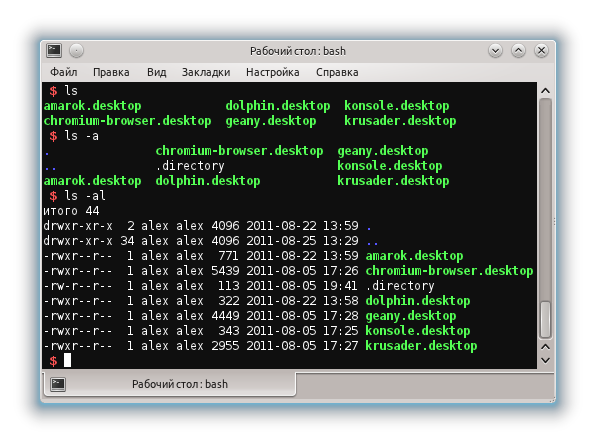
\includegraphics[width=5cm]{files/unix_quickstart/bash.png}
		
		{\color{gray}\tiny Источник картинки: \color{blue}\url{https://habrahabr.ru/post/127084/}}
	\end{center}
\end{frame}

\begin{frame}[fragile]{Начало работы}
	Итак, Вы открыли bash в своём любимом эмуляторе терминала. Скорее всего, Вы увидите примерно такое \emph{приглашение bash}:
	\begin{Verbatim}[commandchars=\\\{\},codes={\catcode`$=3\catcode`^=7\catcode`_=8}]
alex@localhost:~\$
	\end{Verbatim}
	\pause
	Для работы с bash небходимо ввести нужную Вам команду, подождать, пока она выполнится (о завершении предыдущей команды bash проинформирует Вас, напечатав очередное приглашение), ввести следующую команду и так далее. Всё просто! 
\end{frame}

\subsection{Навигация по ФС}

\begin{frame}{Навигация по файловой системе}
	\begin{itemize}
		\item{Наберите команду \texttt{ls} и нажмите \texttt{Enter}. Вы увидите список файлов и каталогов, которые лежат в Вашем домашнем каталоге.}\pause
		\item{Чтобы не захламлять домашний каталог, давайте создадим себе песочницу. Введите команду \texttt{mkdir sandbox}, после чего введите команду \texttt{cd sandbox}.}\pause
		\item{Как Вы могли заметить, приглашение изменилось: теперь вместо тильды \texttt{\~} написано \texttt{sandbox}. Это значит, что \emph{текущий рабочий каталог} изменился.}
	\end{itemize}
\end{frame}

\begin{frame}
	\begin{tikzpicture} [
	thick,
	node distance=3.5cm,
	text height=1.5ex,
	text depth=.25ex,
	auto
	]
	\node[workdir] (home1) {\ttfamily /home/alex};
	
	\pause
	
	\node[workdir,right of=home1] (home2) {\ttfamily /home/alex};
	\node[dir,below of=home2] (sandbox2) {\ttfamily sandbox};
	\path[->] (home2) edge (sandbox2);
	\path[->, draw] (home1) ++(0.5,-2) -- node {\ttfamily mkdir sandbox} ++(2.5,0);
	
	\pause
	
	\node[dir,right of=home2] (home3) {\ttfamily /home/alex};
	\node[workdir,below of=home3] (sandbox3) {\ttfamily sandbox};
	\path[->] (home3) edge (sandbox3);
	\path[->, draw] (home2) ++(0.5,-2) -- node {\ttfamily cd sandbox} ++(2.5,0);
	
	\pause[0]
	\end{tikzpicture}
	
	\vphantom{A}
	
	{\color{gray} Текущий рабочий каталог обозначен более тёмным овалом }
\end{frame}

\begin{frame}
	\begin{itemize}
		\item{Если Вы забыли, в каком каталоге Вы сейчас находитесь, воспользуйтесь командой \texttt{pwd}}\pause
		\item{\textbf{Замечание:} многие команды bash являются сокращениями. Так, \texttt{ls} --- это сокращение от \textbf{l}i\textbf{s}t directory contents (в англоязычной литературе использутся слово \emph{директория} вместо слова \emph{каталог}), \texttt{cd} --- \textbf{c}hange \textbf{d}irectory}, \texttt{mkdir} --- \textbf{m}a\textbf{k}e \textbf{dir}ectory, \texttt{pwd} --- \textbf{p}rint \textbf{w}orking \textbf{d}irectory и так далее.
	\end{itemize}
\end{frame}

\subsection{Создание и удаление файлов}

\begin{frame}[fragile]{Создание и удаление файлов}
	\begin{itemize}
		\item{Итак, создавать каталоги мы уже умеем. Давайте научимся их удалять. Создайте каталог \texttt{foo}, а затем удалите его с помощью команды \texttt{rmdir} (remove directory)}\pause
		\item{Для создания файла подходит команда \texttt{touch}. Создайте с её помощью файл \texttt{bar.txt}}\pause
		\item{Чтобы узнать атрибуты этого файла, наберите команду \texttt{ls~-l}. Параметр \texttt{-l} говорит программе \texttt{ls} печатать атрибуты файла, а не только его имя}
	\end{itemize}
	\begin{Verbatim}[commandchars=\\\{\},codes={\catcode`$=3\catcode`^=7\catcode`_=8}]
-rw-r--r-- 1 alex students 0 июл 18 14:06 bar.txt
	\end{Verbatim}
\end{frame}

\begin{frame}[fragile]
	По умолчанию \texttt{ls} печатает следующие атрибуты:\pause
	\begin{itemize}
		\item{Тип файла (файл, каталог, символическая ссылка и т.д.)}\pause
		\item{Права доступа к файлу}\pause
		\item{Число жёстких ссылок на этот файл (будут рассмотрены позднее)}\pause
		\item{Владелец}\pause
		\item{Группа-владелец}\pause
		\item{Размер файла}\pause
		\item{Дата и время последнего изменения}\pause
		\item{Название файла}\pause[0]
	\end{itemize}
	
	\begin{onlyenv}<1>
		\begin{Verbatim}[commandchars=\\\{\},codes={\catcode`$=3\catcode`^=7\catcode`_=8}]
-rw-r--r-- 1 alex students 0 июл 18 14:06 bar.txt
		\end{Verbatim}
	\end{onlyenv}
	\begin{onlyenv}<2|handout:0>
		\begin{Verbatim}[commandchars=\\\{\},codes={\catcode`$=3\catcode`^=7\catcode`_=8}]
{\color{red}-}rw-r--r-- 1 alex students 0 июл 18 14:06 bar.txt
		\end{Verbatim}
	\end{onlyenv}
	\begin{onlyenv}<3|handout:0>
		\begin{Verbatim}[commandchars=\\\{\},codes={\catcode`$=3\catcode`^=7\catcode`_=8}]
-{\color{red}rw-r--r--} 1 alex students 0 июл 18 14:06 bar.txt
		\end{Verbatim}
	\end{onlyenv}
	\begin{onlyenv}<4|handout:0>
		\begin{Verbatim}[commandchars=\\\{\},codes={\catcode`$=3\catcode`^=7\catcode`_=8}]
-rw-r--r-- {\color{red}1} alex students 0 июл 18 14:06 bar.txt
		\end{Verbatim}
	\end{onlyenv}
	\begin{onlyenv}<5|handout:0>
		\begin{Verbatim}[commandchars=\\\{\},codes={\catcode`$=3\catcode`^=7\catcode`_=8}]
-rw-r--r-- 1 {\color{red}alex} students 0 июл 18 14:06 bar.txt
		\end{Verbatim}
	\end{onlyenv}
	\begin{onlyenv}<6|handout:0>
		\begin{Verbatim}[commandchars=\\\{\},codes={\catcode`$=3\catcode`^=7\catcode`_=8}]
-rw-r--r-- 1 alex {\color{red}students} 0 июл 18 14:06 bar.txt
		\end{Verbatim}
	\end{onlyenv}
	\begin{onlyenv}<7|handout:0>
		\begin{Verbatim}[commandchars=\\\{\},codes={\catcode`$=3\catcode`^=7\catcode`_=8}]
-rw-r--r-- 1 alex students {\color{red}0} июл 18 14:06 bar.txt
		\end{Verbatim}
	\end{onlyenv}
	\begin{onlyenv}<8|handout:0>
		\begin{Verbatim}[commandchars=\\\{\},codes={\catcode`$=3\catcode`^=7\catcode`_=8}]
-rw-r--r-- 1 alex students 0 {\color{red}июл 18 14:06} bar.txt
		\end{Verbatim}
	\end{onlyenv}
	\begin{onlyenv}<9|handout:0>
		\begin{Verbatim}[commandchars=\\\{\},codes={\catcode`$=3\catcode`^=7\catcode`_=8}]
-rw-r--r-- 1 alex students 0 июл 18 14:06 {\color{red}bar.txt}
		\end{Verbatim}
	\end{onlyenv}
\end{frame}

\begin{frame}
	\begin{itemize}
		\item{Для того, чтобы изменить содержимое файла, нужно открыть его любым текстовым редактором, например, gedit (если у Вас стоит Ubuntu, то этот редактор у Вас наверняка есть)}\pause
		\item{Наберите команду \texttt{gedit bar.txt}. Обратите внимание, что в терминале не появляется новое приглашение: bash ждёт, пока Вы закончите работу с gedit}\pause
		\item{После того, как Вы закончили работу с текстовым редактором, \emph{сохранили изменения} и закрыли редактор, в терминале высветится очередное приглашение bash}\pause
		\item{Снова выполните команду \texttt{ls~-l}, чтобы убедиться, что время изменения файла и его размер изменились}
	\end{itemize}
\end{frame}

\begin{frame}
	\begin{itemize}
		\item{Чтобы удалить файл, воспользуйтесь командой \texttt{rm}}\pause
		\item{\textbf{Внимание!} Команда \texttt{rm} \emph{действительно удаляет} файлы, а не перемещает их в корзину. После такой экзекуции восстановление файла не всегда возможно и сопряжено с большими сложностями. Будьте аккуратны!}\pause
		\item{Чтобы переименовать файл, можно воспользоваться командой \texttt{mv}. Например, если набрать \texttt{mv~foo~bar}, то файл \texttt{foo} получит новое имя (если же файла с таким именем не существует, то Вы получите сообщение об ошибке)}\pause
		\item{Если файл \texttt{bar} при этом существовал до исполнения команды, он будет удалён}
	\end{itemize}
\end{frame}

\begin{frame}
	\begin{itemize}
		\item{Вообще, команда \texttt{mv} предназначена для перемещения файлов. Например, если у Вас есть каталог \texttt{subdir}, то команда \texttt{mv bar.txt subdir} приведёт к тому, что файл bar.txt переместится в каталог \texttt{subdir}}
	\end{itemize}
	\begin{tikzpicture} [
	thick,
	node distance=1.5cm,
	text height=1.5ex,
	text depth=.25ex,
	auto
	]
	\pause
	\coordinate (c1);
	\node[workdir,above of=c1] (sandbox1) {\ttfamily sandbox};
	\node[dir,left of=c1] (subdir1) {\ttfamily subdir};
	\node[file,right of=c1] (bar1) {\ttfamily bar.txt};
	\path[->] (sandbox1) edge (subdir1) edge (bar1);
	
	\pause
	\coordinate[right of=bar1] (c2);
	\coordinate[right of=c2] (c3);
	\node[dir,right of=c3] (subdir2) {\ttfamily subdir};
	\node[workdir,above of=subdir2] (sandbox2) {\ttfamily sandbox};
	\node[file,below of=subdir2] (bar2) {\ttfamily bar.txt};
	\path[->] (sandbox2) edge (subdir2);
	\path[->] (subdir2) edge (bar2);
	\path[->,draw] (sandbox1) ++(1.5,0) -- node {\ttfamily mv bar.txt subdir} ++(3,0);
	
	\pause[0]
	\end{tikzpicture}
\end{frame}

\subsection{Запуск исполняемых файлов}
\begin{frame}{Запуск исполняемых файлов}
	Создайте файл \texttt{arglist.sh} и наберите в нём следующий код:
	
	\label{arg_var_example}
	\inputminted[linenos,bgcolor=listing]{bash}{files/unix_quickstart/arglist.sh}\pause
	\vspace*{-\baselineskip}
	
	Теперь выполните команду \texttt{chmod~+x~arglist.sh}. Теперь у нас есть простенький \emph{bash-скрипт}, который можно запустить. \pause
	
	Наберите команду \texttt{./arglist.sh arg1 arg2 arg3} и посмотрите, что выведет этот скрипт. Обратите внимание на символы ``\texttt{./}'': без этих символов bash решит, что требуется системная программа и, не найдя программу с нужным именем, выдаст ошибку.
\end{frame}

\begin{frame}{Аргументы запуска}
	\begin{itemize}
		\item{Скрипт вывел \emph{аргументы запуска} в том порядке, в котором они были указаны, каждый на своей строке}\pause
		\item{Допустим, мы хотим создать файл с названием \texttt{long name with spaces.txt}. Если просто набрать команду \texttt{touch~long~name~with~spaces.txt}, то будут созданы четыре разных файла}\pause
		\item{Чтобы решить эту проблему, нужно поставить двойные кавычки вокруг имени файла: \texttt{touch~"long~name~with~spaces.txt"}}\pause
		\item{Помимо двойных кавычек, иногда используются одинарные: в отличие от двойных, они не поддерживают ни экранирования символов, ни подстановки переменных окружения (о них несколько позже)} 
	\end{itemize}
\end{frame}

\section{Часто используемые утилиты UNIX}

\subsection{GNU Coreutils}
\begin{frame}{Часто используемые утилиты}
	\begin{itemize}
		\item{В UNIX есть большой набор часто используемых утилит, таких как \texttt{ls}, \texttt{chmod}, \texttt{cat}, \texttt{echo} и других}\pause
		\item{Эти утилиты объединены в GNU Coreutils --- пакет, присутствующий во многих UNIX-подобных системах}\pause
		\item{Помимо Coreutils, существует стандарт POSIX (Portable Operating System Interface for Unix), одна из версий которого (а точнее, POSIX.1-2008) описывает список утилит, которые должны присутствовать во всякой POSIX-совместимой системе (этот список является надмножеством Coreutils)}
	\end{itemize}
\end{frame}

\subsection{man}
\begin{frame}{\ttfamily man}
	\begin{itemize}
		\item{Для того, чтобы узнать, как пользоваться той или иной утилитой или функцией, существует программа \texttt{man} (от слова manual --- руководство)}\pause
		\item{Большинство программ, установленных на Вашем компьютере, сопровождаются справочными материалами, которые можно просмотреть с помощью \texttt{man}}\pause
		\item{Для того, чтобы получить информацию по утилите \texttt{ls}, наберите команду \texttt{man ls}} 
	\end{itemize}
\end{frame}

\begin{frame}
	\begin{itemize}
		\item{Справочные страницы man делятся на несколько разделов (о них можно узнать с помощью команды \texttt{man~man})}\pause
		\item{Иногда в разных разделах встречаются страницы с одинаковым заголовком (например, \texttt{stat}). Для того, чтобы прочитать определённую страницу, нужно перед её названием написать номер раздела (например, \texttt{man~2~stat})}\pause
		\item{Для того, чтобы узнать список доступных страниц, нужно воспользоваться командой \texttt{whatis}}\pause
		\item{Для поиска нужной справочной страницы используется утилита \texttt{apropos} (вывод может быть длинным, поиск в Google чаще оказывается результативнее и умнее)}\pause
		\item{Если обе утилиты не работают, возможно, у Вас не настроена база данных man. Чтобы это исправить, запустите команду \texttt{mandb} от имени суперпользователя (\texttt{sudo mandb}, потребует пароль)}
	\end{itemize}
\end{frame}

\section{Программирование на bash}

\subsection{Переменные}
\begin{frame}{Программирование на bash. Переменные}
	\begin{itemize}
		\item{В UNIX-подобных системах существуют так называемые \emph{переменные окружения}. Они используются для того, чтобы регулировать работу программ. Например, переменная \texttt{PATH} содержит список каталогов, в которых bash ищет исполняемые файлы.}\pause
		\item{У каждого процесса есть своя копия этого окружения, которая унаследована от родительского процесса. Благодаря этому у процессов нет возможности изменить глобальные настройки}\pause
		\item{Помимо переменных окружения, есть ещё переменные командной оболочки. Они доступны только в рамках данного экземпляра командной оболочки.}
	\end{itemize}
\end{frame}

\begin{frame}
	\texttt{outer.sh}
	\inputminted[linenos,bgcolor=listing]{bash}{files/unix_quickstart/outer.sh}
	\texttt{inner.sh}
	\inputminted[linenos,bgcolor=listing]{bash}{files/unix_quickstart/inner.sh}
\end{frame}

\begin{frame}
	\begin{itemize}
		\item{Запустив \texttt{outer.sh}, Вы убедитесь, что только во второй раз переменная \texttt{foo} оказалась доступной в другом скрипте}\pause
		\item{Обратите внимание на то, что в обоих скриптах используются строки в двойных кавычках. С одной стороны, если кавычки убрать вообще, то результат работы программы не изменится (теперь вместо одного аргумента \texttt{echo} будет получать несколько, но задача этой утилиты --- вывести все свои аргументы через пробел, если иное поведение не выбрано с помощью ключей). С другой, если заменить двойные кавычки одинарными, то подстановка переменных происходить не будет.}
	\end{itemize}
\end{frame}

\subsection{Условный оператор}
\begin{frame}{Оператор \texttt{if}}
	\begin{itemize}
		\item{В языке bash есть условный оператор \texttt{if}. Он имеет следующий синтаксис:}\pause
	\end{itemize}
	\vspace*{-\baselineskip}
	\inputminted[linenos,bgcolor=listing]{bash}{files/unix_quickstart/if.sh}\pause
	\vspace*{-\baselineskip}
	\begin{itemize}
		\item{\texttt{condition} --- это любая команда. Если эта команда успешно выполнена (с нулевым кодом возврата), условие считается выполненным}\pause
		\item{Блок \texttt{else} не является обязательным}
	\end{itemize}
\end{frame}

\begin{frame}
	\begin{itemize}
		\item{Для работы с условным оператором очень удобно использовать утилиту \texttt{test}. Эта утилита позволяет сравнивать числа, строки, а также проверять наличие некоторых свойств у файлов}\pause
		\item{Например, команда \texttt{if test -f foo.txt; then echo yes; fi} (точки с запятой эквивалентны переносам строк с точки зрения bash) выведет \texttt{yes}, если в текущем каталоге есть обычный файл \texttt{foo.txt}.}\pause
		\item{Команда \texttt{test -f foo.txt} эквивалентна команде \texttt{[ -f foo.txt ]} (обратите внимание на пробелы после открывающей и перед закрывающей скобками)}
	\end{itemize}
\end{frame}

\subsection{Циклы}
\begin{frame}{Цикл \texttt{while}}
	В bash есть цикл \texttt{while}. Его синтаксис похож на синтаксис условного оператора:\pause
	\inputminted[linenos,bgcolor=listing]{bash}{files/unix_quickstart/while.sh}
\end{frame}

\begin{frame}{Цикл \texttt{for}}
	\begin{itemize}
		\item{Гораздо интереснее устроен цикл \texttt{for}. Он используется для итерирования по списку. Его синтаксис выглядит следующим образом:}\pause
	\end{itemize}
	\vspace*{-\baselineskip}
	\inputminted[linenos,bgcolor=listing]{bash}{files/unix_quickstart/for.sh}\pause
	\vspace*{-\baselineskip}
	\begin{itemize}
		\item{Часто в качестве элементов списка выступают слова или строки из вывода какой-нибудь программы. Для этого используется конструкция \texttt{\$(command)}}
	\end{itemize}
\end{frame}

\begin{frame}
	\texttt{sum.sh}
	\inputminted[linenos,bgcolor=listing]{bash}{files/unix_quickstart/sum.sh}\pause
	\vspace*{-\baselineskip}
	\begin{itemize}
		\item{\texttt{seq} позволяет выводить арифметические прогрессии}\pause
		\item{\texttt{let} нужен для целочисленной арифметики}
	\end{itemize}
\end{frame}

\subsection{Аргументы}
\begin{frame}{Аргументы}
	\begin{itemize}
		\item{При запуске скрипта ему можно передать некоторые аргументы. Для доступа к этим аргументам используются специальные переменные вида \texttt{\$0}, \texttt{\$1}, \texttt{\$2} и так далее (нулевая переменная содержит имя запускаемого скрипта)}\pause
		\item{Если нужно получить все аргументы одним списком, можно воспользоваться переменной \texttt{\$@} (см. пример на слайде~\ref{arg_var_example})}\pause
		\item{Если в цикле \texttt{for} не указывать список, по которому нужно проходить, то цикл пойдет по списку аргументов}
	\end{itemize}
\end{frame}

\subsection{Ввод с клавиатуры, оператор case}
\begin{frame}{Ввод с клавиатуры, оператор case}
	\begin{itemize}
		\item{Для ввода с клавиатуры подходит команда \texttt{read}. Замените строчку 3 в предыдущем листинге на такую: \texttt{read~-p~"Enter~N: "{} N}}\pause
		\item{Часто бывает нужно проверить, подходит ли введённый текст под тот или иной шаблон. Можно воспользоваться оператором \texttt{if}, но он плохо приспособлен для такой задачи. Гороздо удобнее использовать оператор \texttt{case}}\pause
		\item{Оператор \texttt{case} по очереди сравнивает переменную с шаблонами. Если находится подходящий шаблон, управление передаётся соответствующему блоку кода}\pause
		\item{Подробнее о шаблонах можно прочитать в разделе Pattern Matching в руководстве к bash}
	\end{itemize}
\end{frame}

\begin{frame}
	\begin{minipage}{0,325\textwidth}
		Синтаксис оператора \texttt{case}
		\inputminted[linenos,fontsize=\tiny,bgcolor=listing]{bash}{files/unix_quickstart/case.sh}
	\end{minipage}
	\begin{minipage}{0,125\textwidth}
		\invisible{qwerty}
	\end{minipage}
	\begin{minipage}{0,525\textwidth}
		\texttt{odd\_even.sh}
		\inputminted[linenos,fontsize=\tiny,bgcolor=listing]{bash}{files/unix_quickstart/odd_even.sh}
	\end{minipage}
\end{frame}

\subsection{Ввод и вывод}
\begin{frame}{Работа с файлами}
	\begin{itemize}
		\item{Часто возникает потребность вводить данные в программу не с клавиатуры, а из файла, а также записывать в файл результат её работы. Для этого используется \emph{перенаправление потоков ввода-вывода}}\pause
		\item{Для того, чтобы заменить стандартный поток ввода файлом, необходимо в конце команды дописать \texttt{<filename} (если такого файла нет, возникнет ошибка)}\pause
		\item{Для того, чтобы перенаправить вывод программы в файл, нужно дописать \texttt{>filename} (если файл отсутствует, он будет создан автоматически)}\pause
		\item{Если необходимо дописать что-то к концу файла, а не перезаписывать его целиком, надо написать \texttt{>{}>filename}}
	\end{itemize}
\end{frame}

\begin{frame}{Конвейеры}
	\begin{itemize}
		\item{Допустим, нам нужно текст, полученный в результате работы программы A, отправить на вход программе B}\pause
		\item{Возможное решение:}
	\end{itemize}
	\vspace*{-\baselineskip}
	\inputminted[linenos,bgcolor=listing]{bash}{files/unix_quickstart/nopipe.sh}\pause
	\vspace*{-\baselineskip}
	\begin{itemize}
		\item{К сожалению, это решение неудобное и не всегда возможное. Поэтому была создана концепция \emph{конвейера}: вместо временного файла в системе выделяется кольцевой буфер (очередь FIFO), в который один процесс пишет, а другой читает из этого буфера. Чтобы так сделать, нужно выполнить команду \texttt{./A~|~./B}}
	\end{itemize}
\end{frame}

\subsection{Массивы}
\begin{frame}{Массивы}
	\inputminted[linenos,bgcolor=listing]{bash}{files/unix_quickstart/arrays.sh}
\end{frame}

\subsection{Функции}
\begin{frame}{Функции}
	\inputminted[linenos,bgcolor=listing]{bash}{files/unix_quickstart/functions.sh}
\end{frame}

\section{Пакеты и пакетные менеджеры. Дистрибутивы}

\begin{frame}{Пакетные менеджеры}
	\begin{itemize}
		\item{В большинстве дистрибутивов Linux и других UNIX-подобных систем для удобства установки, настройки, обновления и удаления программ используются \emph{пакетные менеджеры}}\pause
		\item{Пакетные менеджеры оперируют \emph{пакетами} --- специальными архивами, которые содержат саму программу, файлы, необходимые ей для работы и метаданные для корректной работы самого менеджера (полное название пакета, описание, версия, контрольная сумма, зависимости от других пакетов и так далее)}\pause
		\item{Для хранения пакетов используются специальные сервера, которые называются \emph{репозитории}}
	\end{itemize}
\end{frame}

\begin{frame}
	\begin{itemize}
		\item{В разных дистрибутивах Linux используются разные пакетные менеджеры. Наиболее популярным является RPM --- Red Hat Package Manager. Он используется в RHEL, Fedora, openSUSE, ALT Linux и многих других}\pause
		\item{В дистрибутивах на базе Debian (к ним относится и Ubuntu) используется dpkg, пакеты имеют расширение \texttt{.deb}}\pause
		\item{Существуют и другие, менее распространённые пакетные менеджеры. Так, в Arch Linux используется pacman, в Gentoo --- portage}\pause
		\item{Также пакетными менеджерами являются такие системы, как Play Market и App Store}\pause
		\item{Стоит отметить, что разные пакетные менеджеры не совместимы друг с другом, и использование разных пакетных менеджеров на одной машине --- не лучшая идея}
	\end{itemize}
\end{frame}

\begin{frame}{Дистрибутивы}
	\begin{itemize}
		\item{Во многих дистрибутивах Linux ядро операционной системы и системное ПО тоже распространяется в виде пакета: это позволяет сильно упростить обновление системных компонентов}\pause
		\item{Единственная задача, с которой пакетный менеджер справиться не в состоянии --- это установка новой системы на чистый компьютер. Для этой задачи используются \emph{дистрибутивы}}\pause
		\item{Дистрибутив содержит программу для начальной инициализации системы, программу-установщик и набор пакетов}
	\end{itemize}
\end{frame}

\end{document}
